% =====================================================================
%  DeepScan – MVVM-Architektur (TikZ)
%  ---------------------------------------------------------------------
%  Zwei Nutzungsarten:
%   (A) Eigenständig kompilieren: dieses File direkt mit pdflatex bauen.
%   (B) In die Arbeit einbinden: den \begin{tikzpicture}...\end{tikzpicture}
%       Block in eine figure-Umgebung kopieren, ODER dieses File via
%       \input{thesis-figures/architecture-mvvm-body} laden (dazu den
%       Body in ein separates File auslagern). Benötigte Pakete:
%       \usepackage{tikz}\usetikzlibrary{positioning,fit,backgrounds,arrows.meta}
% =====================================================================
\documentclass[border=8pt]{standalone}
\usepackage{tikz}
\usepackage[scaled]{helvet}\renewcommand\familydefault{\sfdefault}
\usetikzlibrary{positioning,fit,backgrounds,arrows.meta,calc,shadows}

\begin{document}
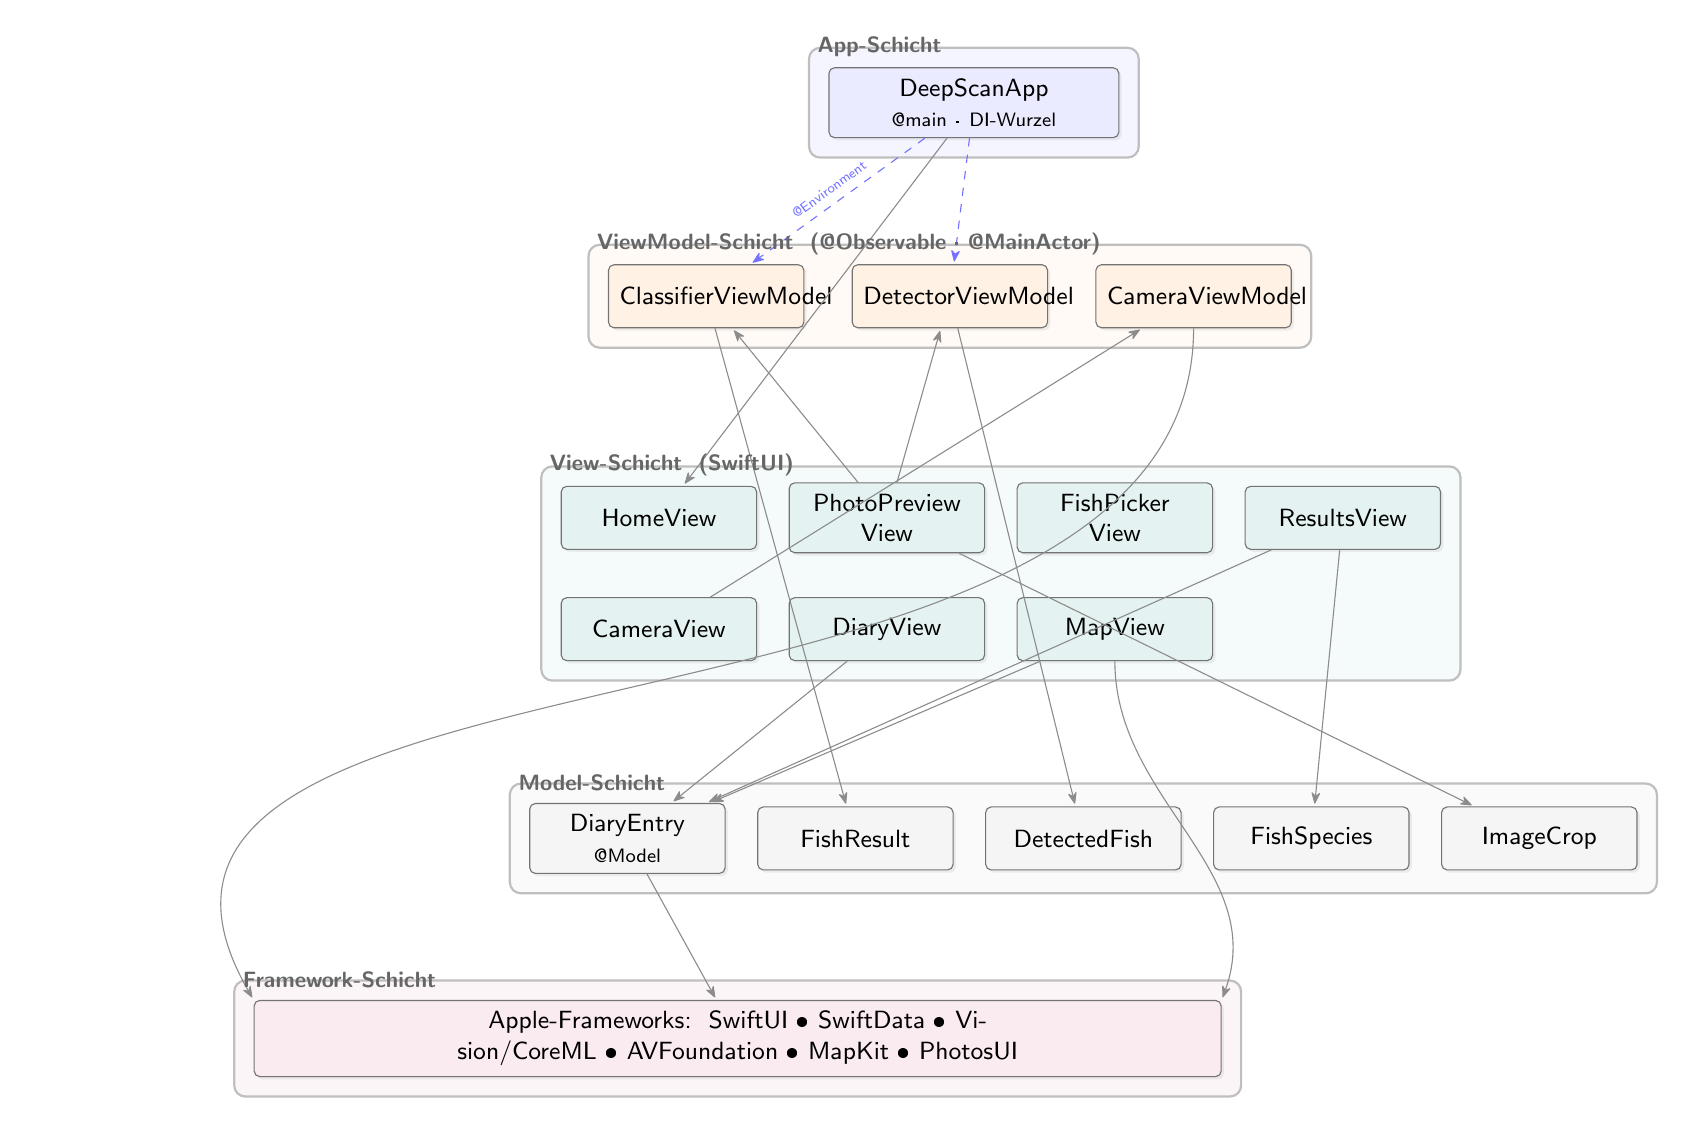
\begin{tikzpicture}[
    font=\small,
    >={Stealth[round]},
    comp/.style={
        draw=black!55, rounded corners=2pt, fill=white,
        minimum height=8mm, inner sep=4pt, align=center,
        text width=22mm, drop shadow={opacity=0.12,shadow xshift=1pt,shadow yshift=-1pt}
    },
    layer/.style={draw=black!25, rounded corners=4pt, inner sep=7pt, line width=0.8pt},
    lbl/.style={font=\footnotesize\bfseries, text=black!60},
    dep/.style={->, draw=black!45, shorten >=1pt},
    inj/.style={->, draw=blue!55, dashed, shorten >=1pt},
]

% ---- App layer -----------------------------------------------------
\node[comp, fill=blue!8, text width=34mm] (app) {DeepScanApp\\\scriptsize @main · DI-Wurzel};

% ---- ViewModel layer ----------------------------------------------
\node[comp, fill=orange!10, below=16mm of app, xshift=-34mm] (cls) {ClassifierViewModel};
\node[comp, fill=orange!10, right=6mm of cls] (det) {DetectorViewModel};
\node[comp, fill=orange!10, right=6mm of det] (cam) {CameraViewModel};

% ---- View layer ----------------------------------------------------
\node[comp, fill=teal!10, below=20mm of cls, xshift=-6mm] (home) {HomeView};
\node[comp, fill=teal!10, right=4mm of home] (preview) {PhotoPreview\\View};
\node[comp, fill=teal!10, right=4mm of preview] (picker) {FishPicker\\View};
\node[comp, fill=teal!10, right=4mm of picker] (results) {ResultsView};
\node[comp, fill=teal!10, below=6mm of home] (cameraV) {CameraView};
\node[comp, fill=teal!10, right=4mm of cameraV] (diary) {DiaryView};
\node[comp, fill=teal!10, right=4mm of diary] (map) {MapView};

% ---- Model layer ---------------------------------------------------
\node[comp, fill=black!4, below=18mm of cameraV, xshift=-4mm] (entry) {DiaryEntry\\\scriptsize @Model};
\node[comp, fill=black!4, right=4mm of entry] (fres) {FishResult};
\node[comp, fill=black!4, right=4mm of fres] (dfish) {DetectedFish};
\node[comp, fill=black!4, right=4mm of dfish] (species) {FishSpecies};
\node[comp, fill=black!4, right=4mm of species] (crop) {ImageCrop};

% ---- Framework layer ----------------------------------------------
\node[comp, fill=purple!8, below=16mm of entry, xshift=14mm, text width=120mm]
    (fw) {Apple-Frameworks:\ \ SwiftUI \textbullet\ SwiftData \textbullet\ Vision/CoreML \textbullet\ AVFoundation \textbullet\ MapKit \textbullet\ PhotosUI};

% ---- Dependencies (selected, top-down) -----------------------------
\draw[inj] (app) -- (cls) node[midway,sloped,above,font=\tiny,text=blue!55]{@Environment};
\draw[inj] (app) -- (det);
\draw[dep] (app) -- (home);

\draw[dep] (preview) -- (cls);
\draw[dep] (preview) -- (det);
\draw[dep] (cameraV) -- (cam);
\draw[dep] (preview) -- (crop);
\draw[dep] (results) -- (species);
\draw[dep] (results) -- (entry);
\draw[dep] (diary) -- (entry);
\draw[dep] (map) -- (entry);
\draw[dep] (cls) -- (fres);
\draw[dep] (det) -- (dfish);

\draw[dep] (entry) -- (fw);
\draw[dep] (cam.south) to[out=-90,in=120] (fw.north west);
\draw[dep] (map.south) to[out=-90,in=70] (fw.north east);

% ---- Layer backgrounds + labels -----------------------------------
\begin{scope}[on background layer]
    \node[layer, fill=blue!4,   fit=(app)] (Lapp) {};
    \node[layer, fill=orange!4, fit=(cls)(det)(cam)] (Lvm) {};
    \node[layer, fill=teal!4,   fit=(home)(results)(cameraV)(map)] (Lview) {};
    \node[layer, fill=black!2,  fit=(entry)(crop)] (Lmodel) {};
    \node[layer, fill=purple!4, fit=(fw)] (Lfw) {};
\end{scope}
\node[lbl, anchor=west] at (Lapp.north west)   {App-Schicht};
\node[lbl, anchor=west] at (Lvm.north west)    {ViewModel-Schicht\ \ (@Observable · @MainActor)};
\node[lbl, anchor=west] at (Lview.north west)  {View-Schicht\ \ (SwiftUI)};
\node[lbl, anchor=west] at (Lmodel.north west) {Model-Schicht};
\node[lbl, anchor=west] at (Lfw.north west)    {Framework-Schicht};

\end{tikzpicture}
\end{document}
